% ===========================================================================
% sar_swarm - schelet de articol IEEE
% Resilient Multi-Robot SAR Coordination over Degraded Networks:
%   rmw_zenoh vs DDS
%
% NOTE de compilare:
%  - Local (fara IEEEtran.cls): schimba prima linie in \documentclass{article}
%    si bibliographystyle in {plain}. Un build.sh poate face fallback automat.
%  - Pe Overleaf / TeX Live complet: lasa IEEEtran (linia de mai jos).
%  - ASCII-only obligatoriu (fara diacritice) - cere IEEEtran/OT1.
% ===========================================================================
\documentclass[conference]{IEEEtran}
% \documentclass{article}   % <-- fallback local daca IEEEtran.cls lipseste

\usepackage{graphicx}
\usepackage{amsmath}
\usepackage{booktabs}
\usepackage{url}

\title{Resilient Multi-Robot Search-and-Rescue Coordination over
Degraded Networks: A Comparison of rmw\_zenoh and DDS}

\author{\IEEEauthorblockN{Alexandru [Nume]}
\IEEEauthorblockA{Institutul de Mecanica Solidelor (IMSAR)\\
Academia Romana, Bucuresti, Romania}}

\begin{document}
\maketitle

% ---------------------------------------------------------------------------
\begin{abstract}
Multi-robot search-and-rescue (SAR) systems must coordinate a drone swarm with
a ground control station (GCS) over networks that are frequently degraded:
packet loss, latency spikes, and partitions. We present a SAR swarm built on
ROS~2 whose mission performance is evaluated systematically under controlled
network degradation, and we compare two middleware transports, rmw\_zenoh and
rmw\_cyclonedds, on the same mission metrics. We introduce an end-to-end
telemetry-age metric and a goodput metric that capture information freshness at
the GCS, beyond round-trip probes. A multi-hop mesh layer recovers telemetry
from drones isolated from the GCS via relay through neighbors. In
software-in-the-loop experiments, goodput degrades monotonically with loss
(1.00 to 0.29 at 70\% loss) while coverage stays robust (0.95 down to 0.85),
and the mesh layer delivers 55\% more telemetry, letting the GCS learn all
victims 26~s earlier under partition. [Transport comparison numbers: from the
ROS campaign.]
\end{abstract}

\begin{IEEEkeywords}
search and rescue, multi-robot systems, ROS 2, network degradation, Zenoh, DDS,
mesh networking
\end{IEEEkeywords}

% ---------------------------------------------------------------------------
\section{Introduction}
Disaster-response robotics increasingly relies on teams of aerial robots that
explore a hazardous area and report findings to human operators. The
communication link between the robots and the GCS is the weakest point: in
collapsed-structure environments it suffers severe attenuation, intermittent
loss, and partitions. Yet most multi-robot SAR evaluations assume near-ideal
connectivity.

This work makes the network the independent variable. We build a ROS~2 SAR
swarm and measure how its mission performance responds to controlled
degradation, and we ask whether the choice of middleware transport
(rmw\_zenoh vs rmw\_cyclonedds) matters under these conditions. Contributions:
\begin{itemize}
\item a reproducible degradation harness (loss, latency spikes, partition,
isolation) with software-in-the-loop and ROS validation;
\item mission-level metrics for information freshness at the GCS (end-to-end
telemetry age, goodput) that round-trip probes miss;
\item a multi-hop mesh layer that recovers telemetry from isolated drones, with
quantified mission impact;
\item a transport comparison of rmw\_zenoh vs DDS on identical mission metrics.
\end{itemize}

% ---------------------------------------------------------------------------
\section{Related Work}
% [DE COMPLETAT cu citarile reale - structura de baza:]
\textbf{Multi-robot SAR and coverage.} Prior work on swarm coverage and
frontier-based exploration assumes reliable communication; degradation is rarely
the controlled variable.

\textbf{ROS 2 middleware and Zenoh.} The ROS~2 middleware abstraction (rmw)
allows swapping DDS implementations; rmw\_zenoh has emerged as an alternative
targeting lossy and constrained networks. Existing benchmarks compare
throughput and latency under ideal conditions; systematic evaluation under SAR
degradation is missing -- the gap this paper addresses.

\textbf{Mesh and FANET routing.} Multi-hop routing for flying ad-hoc networks
builds on metrics such as ETX~\cite{decouto2004}, used in OLSR, B.A.T.M.A.N. and
Babel. We adopt ETX with Dijkstra for the relay layer.

% ---------------------------------------------------------------------------
\section{System Architecture}
The swarm comprises four drones and a GCS. Each drone runs a thin ROS node over
a tested pure-Python core (kinematics, world model, channel model). Drones
explore frontiers, sense free cells and victims, and send periodic telemetry;
the GCS fuses partial maps into a global coverage map and tracks reported
victims. On link loss a drone enters a fallback state machine
(LINKED~$\rightarrow$~LOCAL~$\rightarrow$~RETURN~$\rightarrow$~LOITER) and buffers
telemetry for store-and-forward delivery on reconnection.

\subsection{Degradation model}
Degradation is applied at message reception: each message is delayed
($\mathrm{lat}\pm\mathrm{jitter}$), dropped with probability $\mathrm{loss}$, or
blocked when the link is down. A fault-injector node drives the link state from
a scenario timeline (loss, latency spike, partition, isolation).

\subsection{Mesh layer}
When a drone lacks a direct link to the GCS, the mesh layer routes its telemetry
through neighbors. Link quality maps to a packet delivery ratio (PDR) via a
log-distance radio model; the routing metric is the Expected Transmission Count
$\mathrm{ETX}=1/(\mathrm{PDR}_{fwd}\cdot\mathrm{PDR}_{rev})$~\cite{decouto2004};
shortest paths to the GCS are computed with Dijkstra over ETX, and forwarding is
directed hop-by-hop with deduplication and TTL.

% ---------------------------------------------------------------------------
\section{Metrics}
Beyond coverage and victims-found, we report: \emph{end-to-end telemetry age}
(the age of mission information when it reaches the GCS, p50/p95), distinct from
round-trip probe RTT because it measures the real mission data flow;
\emph{goodput} (delivered/offered telemetry); and \emph{fallback time} (drone-
seconds spent isolated from the GCS).

% ---------------------------------------------------------------------------
\section{Experimental Results}

\subsection{Degradation produces a measurable gradient}
Table~\ref{tab:scenarios} reports mission metrics across scenarios (SIL,
seed~11). Goodput decreases monotonically with loss, from 1.00 (baseline) to
0.29 at 70\% loss, while end-to-end telemetry p95 rises from 53 to 121~ms.
Coverage stays robust ($\sim$0.95) through 30\% loss, dropping to 0.85 only at
70\%. Different degradation types have distinct signatures: a latency spike
pushes e2e to 2.3~s while keeping goodput high; a partition pushes e2e p95 to
18.5~s (store-and-forward after reconnection) with 80 drone-seconds in fallback.

\begin{table}[t]
\caption{Mission metrics across degradation scenarios (SIL, seed 11).}
\label{tab:scenarios}
\centering
\begin{tabular}{lcccc}
\toprule
Scenario & Coverage & e2e p95 [ms] & Goodput & Fallback [d$\cdot$s]\\
\midrule
baseline        & 0.95 & 53    & 1.00 & 0\\
loss\_30        & 0.95 & 85    & 0.69 & 0\\
loss\_70        & 0.85 & 121   & 0.29 & 0\\
gcs\_delay\_spike & 0.96 & 2296 & 0.98 & 0\\
partition\_2v2  & 0.92 & 18546 & 0.95 & 80\\
drone\_isolation & 0.95 & 77   & 0.95 & 35\\
\bottomrule
\end{tabular}
\end{table}

\begin{figure}[t]
\centering
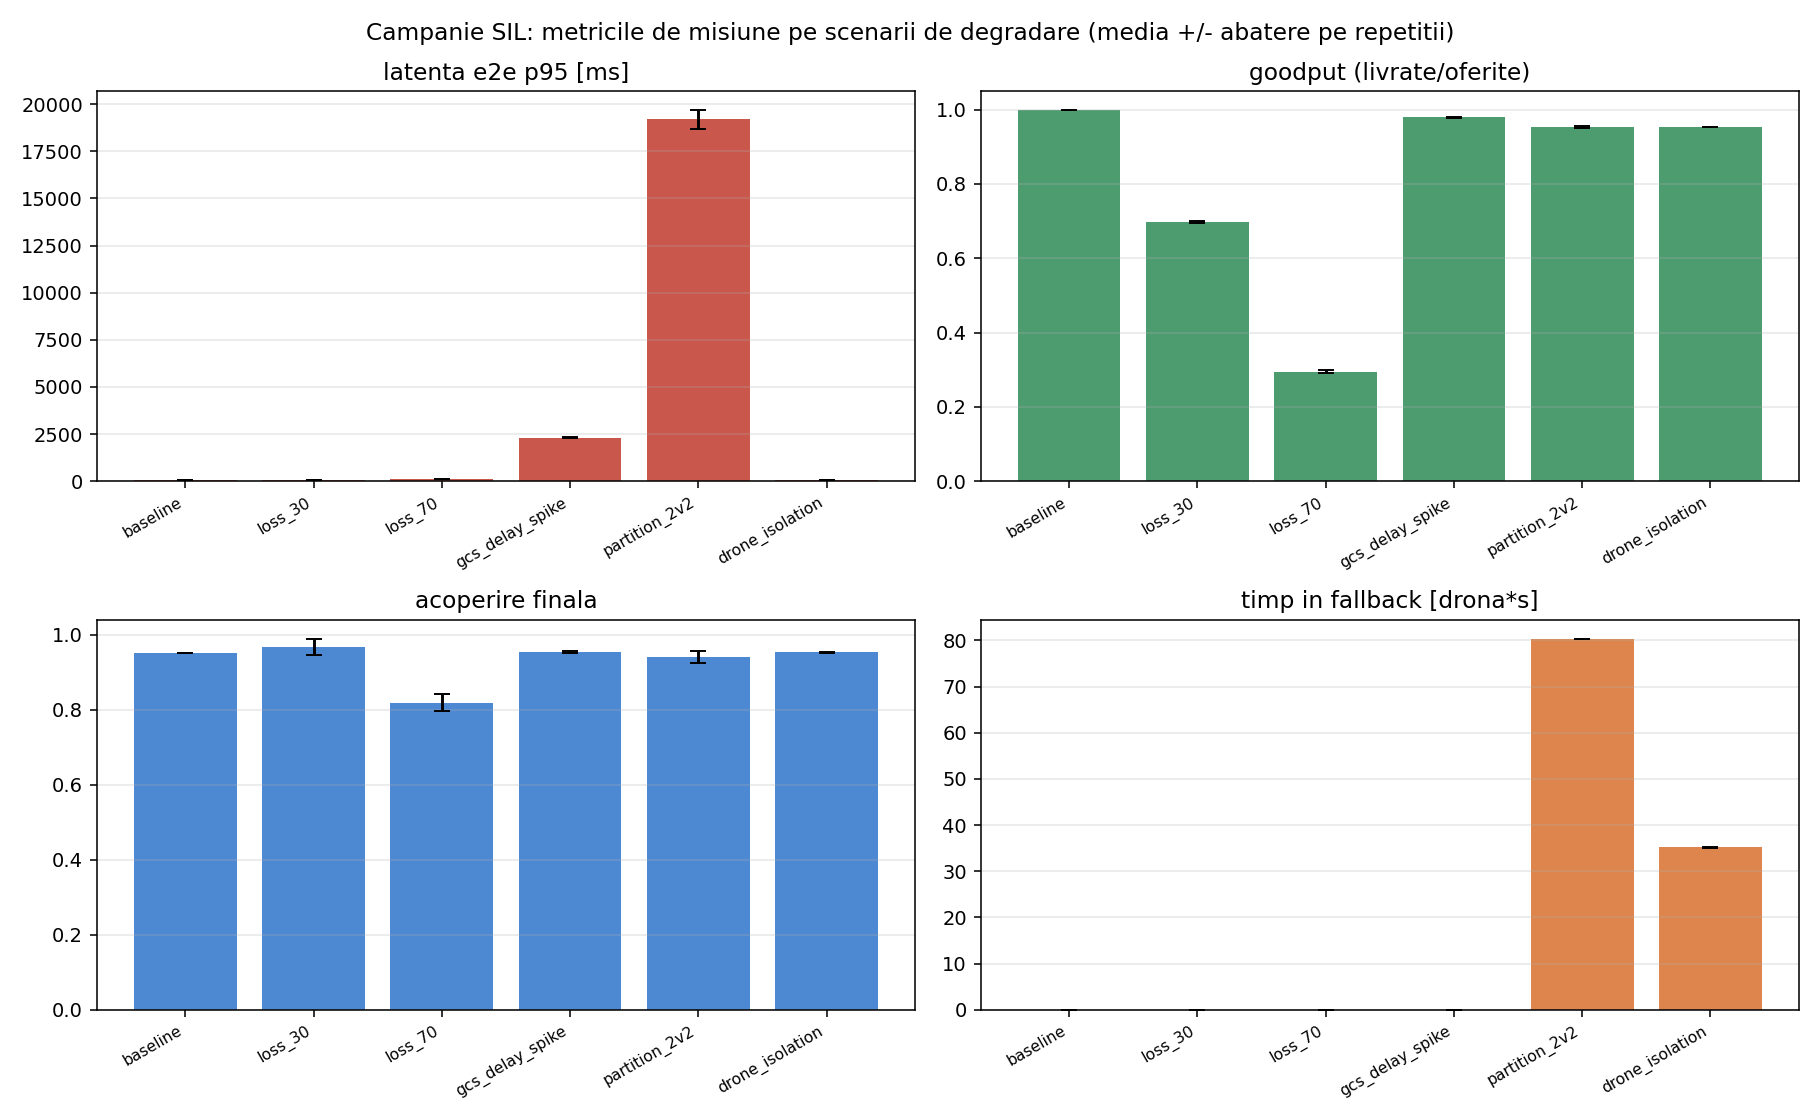
\includegraphics[width=\columnwidth]{campaign_metrics.png}
\caption{Mission metrics across scenarios (mean $\pm$ std over repetitions).}
\label{fig:campaign}
\end{figure}

\subsection{Mesh layer recovers isolated telemetry}
Under the mesh\_relay scenario (two drones lose the direct GCS link but keep
neighbor links), the mesh layer delivers 55\% more telemetry, and the GCS learns
all victims 26~s earlier (64~s vs 90~s, Fig.~\ref{fig:mesh}). The mesh does not
change \emph{how many} victims are found but \emph{how soon} the rescue team
learns of them.

\begin{figure}[t]
\centering

\includegraphics[width=\columnwidth]{mesh_mission_victims.png}
\caption{Victims known at the GCS over time, with vs without the mesh layer.}
\label{fig:mesh}
\end{figure}

\subsection{Transport comparison: rmw\_zenoh vs DDS}
% [DE COMPLETAT cu datele din campania ROS reala]
On identical mission metrics under the same degradation, we compare rmw\_zenoh
and rmw\_cyclonedds across terrain profiles. [Insert Fig.~rmw\_e2e and the
end-to-end latency / goodput differences measured on the ROS campaign.]

% ---------------------------------------------------------------------------
\section{Conclusion}
Making the network the independent variable reveals that a ROS~2 SAR swarm
remains effective under moderate degradation, that information-freshness metrics
expose effects invisible to round-trip probes, and that a multi-hop mesh layer
materially shortens the time-to-knowledge under partition. [Transport
conclusion: from the ROS comparison.]

% ---------------------------------------------------------------------------
\begin{thebibliography}{1}
\bibitem{decouto2004}
D.~S.~J. De Couto, D. Aguayo, J. Bicket, and R. Morris,
``A high-throughput path metric for multi-hop wireless routing,''
in \emph{Proc. ACM MobiCom}, 2003.
% [DE ADAUGAT: citarile pentru SAR swarm, ROS 2 rmw, Zenoh, FANET routing]
\end{thebibliography}

\end{document}
